\documentclass[a4paper,11pt]{article}

\pdfminorversion=4

\usepackage{cmap}
\usepackage[utf8]{inputenc}
\usepackage[T1]{fontenc}
\usepackage{lmodern}
\usepackage{geometry}
\usepackage{graphicx}
\usepackage{amsmath}
\usepackage{amssymb}
\usepackage{xcolor}
\usepackage{listings}
\usepackage{float}
\usepackage{hyperref}

\geometry{margin=2.4cm}
\setlength{\parindent}{0pt}
\setlength{\parskip}{0.65em}
\setlength{\emergencystretch}{2em}
\renewcommand{\abstractname}{Abstract}
\renewcommand{\figurename}{Figure}

\lstset{
  basicstyle=\ttfamily\small,
  breaklines=true,
  frame=none,
  backgroundcolor=\color{gray!8},
  xleftmargin=1em,
  xrightmargin=1em,
}

\title{Software Architecture as a Layered Representation\\
  \large Analyzing Software Architecture with S202}
\author{Johannes Weigend}
\date{Revised version, November~24,~2026}

\begin{document}

\maketitle

\begin{abstract}
S202 computes a hierarchical layered representation of Java systems from
bytecode. The tool derives an architectural hypothesis from the observed class
dependencies by letting every package container order its direct children
independently, distinguishes two kinds of cycles — class-level cycles and
package-level cycles — makes both visible as separately toggled findings, and
checks the finished representation redundantly against consistency rules. This
document describes typical errors in the computation of such layouts, explains
the conceptual solution, and shows how the representation can be used as a
working tool for refactoring planning.
\end{abstract}

\section{Introduction}

At least since the layered models for operating systems in the late 1960s,
software architecture has been represented as a layered dependency structure.
The principle is still relevant today: in cloud-native architectures it helps
to order technical dependencies between services, platforms, and
infrastructure; in domain-driven design it helps to make domain boundaries and
dependencies between bounded contexts visible. The basic idea is simple: an
element that uses another element is placed above the element it uses.
Dependencies therefore run from top to bottom. Edges in the opposite direction
stand out because they often indicate cycles, unwanted coupling, or a broken
layering order.

Such vertically aligned graphs help to understand systems and to detect
anomalies in their dependencies. A simple example is provided by the Java tool
\texttt{jdeps} and the Graphviz tool \texttt{dot}: \texttt{jdeps} extracts
class dependencies from a JAR, and \texttt{dot} turns them into a directed
graph.

\newpage

Figure~\ref{fig:acyclic-levels} shows an acyclic example from the Example JAR
of the S202 codebase. It was created with \texttt{jdeps} and \texttt{dot}. The
JAR contains nine classes in three packages: \texttt{example},
\texttt{example1}, and \texttt{example2}.

\begin{figure}[H]
  \centering
  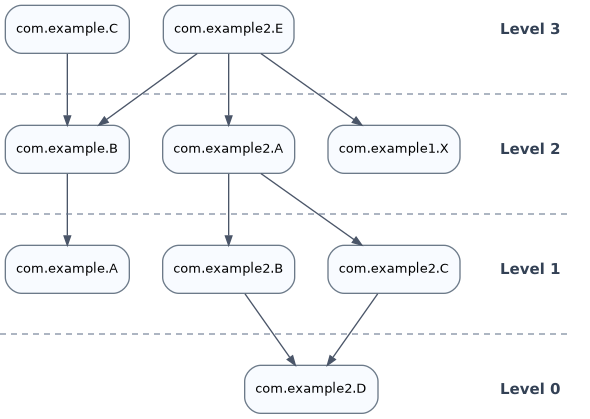
\includegraphics[width=0.75\textwidth]{figures/test-example-classgraph-acyclic-levels.png}
  \caption{Acyclic example from \texttt{test-example-1.0.0.jar}.}
  \label{fig:acyclic-levels}
\end{figure}

The arrows between the boxes are dependencies between classes by invocation or
use. In the example, \texttt{com.example.B} uses class
\texttt{com.example.A}, abbreviated as $B \to A$. The horizontal lines were
added manually and visualize the levels of the layering. Level~0 forms the
foundation; higher levels represent elements that depend on elements below
them.

This kind of representation is useful and widely used. As a visualization of
real applications, however, it has three practical problems:

\begin{enumerate}
  \item Many arrows make the graph hard to read even for medium-sized
        applications.
  \item The package structure is spread across several levels and does not
        form a visible grouping.
  \item With cyclic dependencies, the cycle must be broken for level
        computation so that any vertical order can be created at all. The
        original dependency graph remains unchanged; only the derived DAG
        (\emph{Directed Acyclic Graph}) used for level computation is changed.
        The decisive question is therefore which edge is excluded from this
        computation, because exactly this edge later appears as a break in the
        computed order.
\end{enumerate}

\section{S202 as a Hierarchical Layered Representation}

With the open source tool S202, we address these problems directly. S202 does
not simply replace the flat class graph with an improved representation. It
replaces it with a hierarchical architectural hypothesis: packages remain
visible as containers, and inside each container, packages or classes are
ordered by their dependencies.

The arrows can be shown optionally. In the normal case, however, the vertical
order alone should make it understandable which parts of the application are
higher up and which parts serve as the foundation. Unwanted dependencies
therefore do not appear merely as a single line in a large network, but as a
break in an expected layering order.

Unlike the flat class graph, S202 structures levels hierarchically through the
package structure. Each package orders its direct children, that is,
subpackages or classes, according to their local dependencies. The package
structure remains visible instead of being pulled apart by the class graph.

\begin{figure}[H]
  \centering
  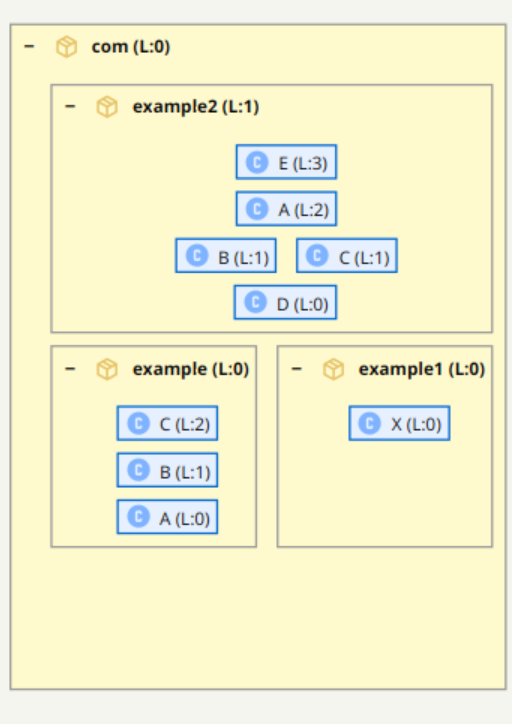
\includegraphics[width=0.55\textwidth]{figures/s202-dependencies-acyclic.png}
  \caption{S202 representation of the acyclic example: packages remain visible
  as containers, classes are ordered within their container, and arrows can be
  shown when needed.}
  \label{fig:s202-acyclic}
\end{figure}

The example shows the package structure below the outer package
\texttt{com}: \texttt{example}, \texttt{example1}, and \texttt{example2} are
subtrees of this container. In the \texttt{example2} subtree there is a
non-trivial internal class structure; at the same time, the overarching
structure shows that \texttt{example2} depends on \texttt{example} and
\texttt{example1}. At class level, \texttt{example2} has the order
$E \to A \to (B \mid C) \to D$. The representation deliberately abstracts
from individual edges. Whether \texttt{A} has a dependency to \texttt{B}, to
\texttt{C}, or to both is less important for the coarse architectural view
than the layering of the package. This abstraction is exactly what keeps large
relationship networks readable.

The idea is not new. The commercial product Structure101 already had a very
similar representation. However, there is no open implementation and no
technical documentation that explains how such a layout can be computed
reliably. S202 closes this gap as an open source tool under the Apache license.

This document describes the typical pitfalls in implementing such a layout and
shows a solution that eliminates many of these problems cleanly at the
conceptual level.

\section{Typical Errors in Computing Layers}

Figures~\ref{fig:acyclic-levels} and~\ref{fig:s202-acyclic} deliberately show
a simple, acyclic example. In this case the layering is unambiguous:
\texttt{E} is above \texttt{A}, \texttt{A} is above \texttt{B} and
\texttt{C}, and both are above \texttt{D}. There is no feedback, so no edge
has to be selected and ignored for level computation.

In real applications this case is the exception rather than the rule. As soon
as classes or packages depend on each other cyclically, a normal graph pass is
no longer sufficient. This is where the interesting errors begin: the
representation may still look plausible, but the computed levels are no longer
stable or no longer explainable in architectural terms.

In the following sections, the term SCC plays a central role. An SCC
(\emph{Strongly Connected Component}) is a set of nodes in which every node can
reach every other node through directed dependency paths. In such a cycle, not
all dependencies can run downward at the same time.

A correct layered layout must therefore satisfy several requirements at once:

\begin{enumerate}
  \item If $A \to B$, then $A$ must be placed above $B$.
  \item Packages must remain visible as containers. A package must not be moved
        accidentally just because a single contained class has a high class
        level.
  \item Classes or packages that form an SCC must be handled explicitly,
        because in a cycle not all edges can run downward at the same time.
\end{enumerate}

Each requirement is manageable in isolation. Together, however, they create a
circular dependency system between the levels of computation themselves: class
levels influence visible positions, package containers structure these
positions, and SCCs force corrections to an order that would already have been
computed without cycle handling. This is the source of the typical failure
modes.

\subsection{Retroactive Correction}

Retroactive correction means here that a structure discovered later forces a
subsequent change to levels that have already been computed.

A naive algorithm iterates over the classes and assigns levels directly. It
first sees class \texttt{A}, assigns its level, and thereby also lifts the
package of \texttt{A}. Later it finds class \texttt{B} and discovers that
\texttt{A} and \texttt{B} belong to the same SCC and must be handled together.
Now \texttt{A} would have to be corrected, and with it its package and possibly
further packages that depend on it.

The problem is not the correction itself. The problem is that parts of the
layout have already been treated as finished at that point. An algorithm that
mixes cycle detection and level assignment has to change, retroactively, places
that it had already left behind.

\subsection{Order-Dependent Results}

Classes come from JARs. The order in which a tool sees classes follows not the
architecture, but the packaging order of the JAR, the module order, the build
tool, or filesystem details. If an algorithm handles cycles as a side effect
during this traversal, the result depends on this accidental order.

This is dangerous because the error does not have to be immediately visible.
The graph may still look roughly correct. Nevertheless, the same codebase can
receive different levels depending on the build configuration.

\subsection{Mixed Class and Package Levels}

One obvious mistake is to derive the level of a package from the highest level
of the classes it contains. This sounds plausible, but it mixes two different
questions: where a class lies in the class graph, and where a package lies in
the architectural hypothesis.

A package is not architecturally high just because it happens to contain a
highly placed class. The central rule is:

\begin{quote}
  Package levels are derived from package dependencies, not from the maximum
  height of individual classes.
\end{quote}

This sounds trivial, but it is not. Precisely because packages are containers
for classes, it is tempting to derive their position from the classes they
contain. That is exactly how two levels get mixed that must remain separate.
Only when package levels are derived from package dependencies do packages
remain stable architectural units. Otherwise a single outlier class is enough
to lift the package to the wrong level and thereby make the container
unusable, even though that container is supposed to provide orientation.

The same mixing exists one level up. If a package's level is computed from a
graph that also carries the dependencies among its own sub-packages, a package
rises merely because it is deeply layered inside. A package that contains
everything it uses belongs on level~0, no matter how its children relate to one
another. The complete rule therefore reads: an element's level arises only from
dependencies that leave its own interior.

\subsection{The Big Lake}

The formally clean answer to cycles is: all elements of an SCC receive the
same level. For small cycles this is acceptable. In real systems, however,
SCCs can become very large. Then hundreds or thousands of classes end up on
the same level. The layering disappears; what remains is a flat block.

The cycle is then correctly detected, but no longer usefully visualized. A tool
must therefore be able to break large SCCs. The decisive point is that the cut
edges must not disappear. They must remain visible, because they explain why
the computed order is only an architectural hypothesis.

\section{Two Kinds of Cycles}

S202 distinguishes two fundamentally different kinds of cycles and makes both
visible as separately toggled overlays:

\begin{description}
  \item[Class cycles (red)] Strongly connected components at the class level.
        Two or more classes that depend on each other directly or transitively
        form such a cycle. Class cycles reveal implementation-level coupling
        that prevents a strict linear order of individual classes. They are
        detected by Tarjan's algorithm on the class dependency graph.
  \item[Package cycles (orange)] Tangles inside a container. A container is a
        package (or the root); its children are the classes and sub-packages it
        directly contains. Two children depend on each other as soon as any
        class in the subtree of one uses a class in the subtree of the other.
        When children of a container form a cycle this way and at least one of
        them is a package, there is a package cycle, regardless of which
        concrete classes inside them are responsible. Package cycles reveal
        architectural-level coupling: the package structure itself has circular
        dependencies. A cycle consisting only of classes of the same package is
        not a package cycle; the red overlay shows it.
\end{description}

The distinction matters because the two kinds answer different questions:

\begin{itemize}
  \item A \emph{class cycle} shows where individual classes need to be
        untangled. Breaking it often requires moving a method, extracting an
        interface, or inverting a dependency between two specific classes.
  \item A \emph{package cycle} shows where package boundaries themselves are
        broken. Resolving it may require a larger restructuring — merging two
        packages, introducing a new one, or redefining the module split
        entirely.
\end{itemize}

A package cycle can exist even when no individual class cycle is visible —
for example, when two packages call each other through different classes that
are each individually acyclic. Conversely, a class cycle contained entirely
within a single package does not necessarily imply a package cycle.

Because the two overlays answer different questions, S202 keeps them as
independent switches. Activating both at the same time is possible and useful
when looking for the root cause of an architectural problem, but each overlay
is also meaningful on its own: the package-cycle overlay reveals the
structural shape of the problem, while the class-cycle overlay reveals the
concrete edges that cause it.

\section{The Container as the Unit of Ordering}

The solution chosen by S202 is to separate analysis, ordering, and
presentation consistently. The class graph remains the raw model of the actual
dependencies. It is not modified just because a layered representation needs
a DAG. Instead, S202 derives additional views from this graph: SCCs for cycle
detection, a weighted sibling graph per container for ordering, and a
hierarchical UI structure for presentation.

Architectural hypothesis here does not mean a claimed target architecture. It
means an as-is architecture derived from the observed dependencies: the order
that most closely corresponds to the existing code and its dependencies,
without hiding where this order is broken by cycles or back edges.

The unit of ordering is the container. Every package orders its direct
children — classes and sub-packages alike — solely by the dependencies that
run between those children. What happens inside a child is that child's
business; what leaves the container is the business of its parent. Structure101
builds its \emph{Levelized Structure Maps} by the same rule. It is the decisive
step: a class dependency is counted exactly once, namely in the container that
holds both endpoints as children of different subtrees. There is no global
package order from which the local one would be derived, and consequently no
local order that could contradict a global one. A package stays stable as a
container because only its relations to its siblings determine its position.
At the same time, the container order provides a criterion for not choosing
back edges arbitrarily, but for marking them as concrete violations of the
expected order.

The error modes described above thus disappear not through a single
algorithmic trick, but through a clear responsibility: every container decides
for itself and finally. First the dependencies are analyzed, then a plausible
order is determined per container, then the visible structure is built, and
finally it is checked whether the representation keeps its own promise.

\section{From Class Dependencies to Container Ordering}

In S202, the flat class graph is not the visible layout model. It is an
analysis artifact: it serves to capture concrete dependencies, detect SCCs,
and assign every dependency to the container that decides its direction. The
visible S202 graphic then arises from the package structure and the order
inside each container.

A class dependency arises from a method call or a method reference, from an
instantiation, from inheritance, or from a pure type reference: a field,
parameter, or return type, a type argument, a cast, an annotation, a caught
exception. All of these count alike, because in none of these cases does the
code compile without the other class. How much it takes to remove the
dependency is a separate question, and it is answered by the weight. Nested,
local, and anonymous classes are not nodes of their own: what they depend on and
what depends on them counts for the class that encloses them.

For every class dependency $X \to Y$, S202 determines the deepest container
that holds both $X$ and $Y$, and the two children of that container whose
subtrees contain $X$ and $Y$. The dependency becomes an edge between these two
siblings — and only there:

\begin{lstlisting}
com.a.X -> com.b.c.Y    container com     edge com.a   -> com.b
com.a.X -> com.a.Y      container com.a   edge com.a.X -> com.a.Y
com.a.X -> com.a.b.Y    container com.a   edge com.a.X -> com.a.b
\end{lstlisting}

The weight of a sibling edge is the sum of the method calls of all class
dependencies projected onto it; a dependency without calls -- inheritance or a
pure type reference -- contributes a fallback weight of~1. Nothing is propagated: neither the source nor the target
side is multiplied along the ancestor chain. The number of edges is bounded by
the number of class dependencies, and every dependency has exactly one place
where its direction is decided. Classes and packages are equal nodes in this
graph; a class directly in a package and a sub-package of the same package are
ordered against each other.

Cycles in a sibling graph are the tangles of that container. Before level
computation, the graph must be acyclic. When siblings form an SCC, S202 uses a
rank measure to assess whether a sibling tends to use others or tends to be
used by them:

\[
  rank(S) = \frac{out(S) - in(S)}{\max(1,\; out(S) + in(S))}
\]

$out(S)$ is the sum of the edge weights from $S$ to other members of the same
SCC, $in(S)$ the sum of the edge weights from those members to $S$. A positive
rank means: the element uses more than it is used; it tends to belong at the
top. A negative rank means: the element is rather used and tends to belong at
the bottom.

Inside an SCC, all edges $S \to T$ with $rank(S) < rank(T)$ are cut — that
is, all edges that run against the dependency flow. No threshold is used: any
measurable rank difference is sufficient justification for a cut. If all ranks
inside an SCC are equal, the topology provides no directional information. In
that case all internal edges are removed, and the levels of the affected nodes
arise solely from dependencies outside the former SCC. If there are no such
dependencies either, the nodes remain on the same level — as true peers
without a justifiable order.

Both kinds of cuts are applied iteratively: after each pass the SCCs are
recomputed, and for remaining residual SCCs the ranks are recalculated over
their members. The procedure ends when no SCC with at least two members
remains. Symmetry detection is based on the rank measure, not on comparing
weights: an SCC in which all edges carry the same weight is not necessarily
symmetric, because different in- and out-degrees produce different ranks
despite equal weights. The cut sibling edges are the \emph{container back
edges}. Structure101 looks for a smallest possible set of feedback edges at
this point; the rank cut is a deterministic substitute without any claim of
minimality. It is order-independent because all elements are processed in
sorted order.

After this cycle handling, S202 computes the levels on the resulting DAG.
Level~0 consists of the siblings that use no other sibling. Every other
sibling lies one level above the highest sibling it directly uses. This
produces the transitive layering: from $B \to A$ and $C \to B$ follows $A$ on
level~0, $B$ on level~1 and $C$ on level~2, even if no direct edge $C \to A$
exists.

This rule — known as \emph{longest-path} or \emph{ASAP levelization} —
anchors every element as low as possible, directly above its deepest
dependency. It matches the invariant Structure101 documents for its Levelized
Structure Maps: every element depends on at least one element on the level
immediately below. The alternative of pulling every element flush
\emph{beneath its consumer} instead (ALAP) would break that invariant, since a
gap could open between an element and its nearest dependency.

One consequence is accepted deliberately: siblings with the same role but
dependency chains of different depth land on different levels. If several
adapters sit above the same application layer, but one of them additionally
sits above a shared utility package, that one is placed one level higher than
the others — levelization measures dependency depth, not architectural role.

The \emph{localLevel} computed this way is the architectural hypothesis. It
determines the position of every element inside its container, and the chain
of localLevels from the root down to the element is the order against which
violations are measured. It is deliberately local: it compares siblings only.

In addition, S202 maintains a global \emph{architectureLevel} for every
element. It measures how deep the dependency chain below an element really is
and is therefore a measure of its complexity; the height in the 3D view and
the ring of the hexagonal view are based on it. The \emph{architectureLevel}
of a class is its longest-path depth in the class graph. Only the
\emph{level cuts} are set aside: back edges that lie inside a class cycle. A
back edge that merely runs against the order of two packages, without closing
a class cycle, is a real acyclic dependency and still counts. The
\emph{architectureLevel} of a package follows the same rule one level up: it
is its longest-path depth in a package graph in which $P$ depends on $Q$
whenever a non-back-edge leads from the subtree of $P$ into the subtree of $Q$
and neither package contains the other. Both graphs are acyclic by
construction. A package is thus never lifted by its own interior: whoever
contains everything it uses stands on level~0. The global level influences
neither the layout nor the detection of violations.

\section{From Class Cycles to Back Edges}

Figure~\ref{fig:cyclic-class} shows a cyclic example from the Example JAR as a
classic class graph. The two subgraphs for Notification and Payment each
contain feedback.

\begin{figure}[H]
  \centering
  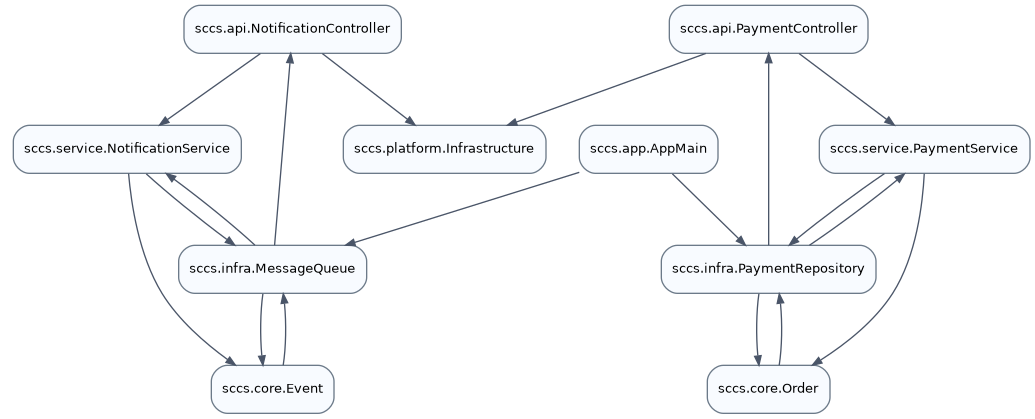
\includegraphics[width=0.9\textwidth]{figures/test-example-classgraph-cyclic.png}
  \caption{Cyclic example from \texttt{test-example-1.0.0.jar}. In every cycle,
  at least one edge must be cut for level computation.}
  \label{fig:cyclic-class}
\end{figure}

The marked cyclic areas are two non-trivial SCCs: one in the Notification part
of the example, with controller, service, message queue, and event classes, and
one in the Payment part, with controller, service, repository, and order
classes. The established procedure for finding such components is Tarjan's
algorithm.

In the cyclic case, the class graph therefore raises the technical question:
which edge must be ignored so that the SCC becomes a computable DAG again for
level assignment? The class graph alone does not provide an architectural
criterion for that. The container order provides it: a class dependency is a
back edge exactly when its projection in its container is a cut sibling edge.

A class cycle that lies inside one package is cut inside that package — there
the classes themselves are the siblings. A class cycle that runs through
several packages appears in the common parent container as a tangle between
packages and is cut there; inside the packages involved, only the edges with
both endpoints inside still count. The retroactive correction from the
catalogue of errors cannot arise this way: no container has to revise a
decision of another one.

From this follows a property that can be proven: every class cycle contains
at least one back edge. In the deepest container that holds all classes of the
cycle, it projects onto a cycle between siblings, and there at least one edge
was cut. For the global class level it is therefore sufficient to set aside
the back edges inside class cycles~-- the \emph{level cuts}. The class graph
is acyclic afterwards; level computation needs no further cycle handling and
no special cases.

Back edges outside class cycles, by contrast, stay in the level computation.
Two packages can use each other through different classes without any class
cycle arising. The edge against the package order is then a violation in the
picture, but still part of the real dependency depth of its class.

All back edges are recorded as \emph{classBackEdge} findings and remain
visible as dashed violation edges.

\begin{figure}[H]
  \centering
  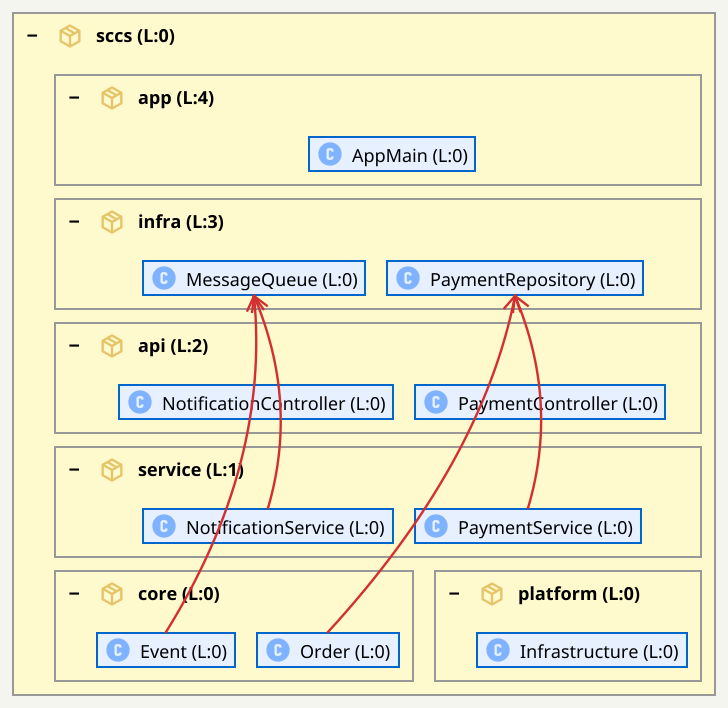
\includegraphics[width=0.6\textwidth]{figures/s202-dependencies-cyclic.png}
  \caption{Cyclic example in the S202 representation. The dashed edges are
  violations: they run against the computed container order and remain visible
  findings of the architectural hypothesis. All four dashed edges are back
  edges: projections of the sibling edges \texttt{core}$\to$\texttt{infra} and
  \texttt{service}$\to$\texttt{infra} cut in the container \texttt{sccs}.}
  \label{fig:s202-cyclic}
\end{figure}

The terms back edge and violation describe different roles of the same edges:

\begin{description}
  \item[Back edge] A class dependency whose projection in its container was cut
        while breaking a tangle. It belongs to cycle handling. If it also lies
        inside a class cycle, it is a level cut and is set aside for the global
        class level.
  \item[Violation] A concrete dependency that runs upward in the computed
        order. What counts here is the \emph{nested} order, not a flat global
        level: the \emph{localLevel} chains of both endpoints are compared from
        the outermost shared container downward, and the direction is decided
        by the first container in which they differ (called \emph{visual rank}
        in the code). Every violation is a back edge, because outside the cut
        edges all sibling edges run downward. Conversely, a back edge runs
        upward or sideways; only when a second path inside a tangle already
        fixes the direction can a cut edge end up pointing downward, and then it
        is not a visible violation. Conceptually, a violation remains the
        visible deviation from the ordering, while a back edge describes the role
        of the edge in cycle handling.
\end{description}

S202 therefore does not hide the cycle. Edges classified as back edges remain
visible as violations because they explain why the container order does not
fully match the concrete class dependencies. This makes the deviation
traceable rather than arbitrary.

\section{Redundant Consistency Checking}

The steps described so far already show why the implementation is prone to
errors. It is not enough to secure individual algorithms with isolated unit
tests. Many errors arise only from the interaction of the data: concrete class
dependencies, package structure, SCCs, aggregated package weights, and local
layout positions influence one another.

S202 therefore checks more than individual computation steps. After the full
pipeline has run, the finished result is checked redundantly against
consistency rules. These rules do not recompute the layout and do not correct
anything. They only read the result and ask whether the generated
representation is internally consistent.

The check consists of five rules:

\begin{enumerate}
  \item \textbf{Class graph:} For every class dependency $A \to B$ that is not
        a level cut, $A$ is on a higher level than $B$, and every level cut is
        a back edge. There are no further exceptions, because the class graph
        without level cuts is acyclic.
  \item \textbf{Container:} In every container, every sibling edge that was not
        cut runs from a higher to a lower \emph{localLevel}. This is the promise
        of the representation itself.
  \item \textbf{Back edges only in tangles:} Every cut sibling edge connects
        two members of the same container tangle. Nothing is cut outside cycles.
  \item \textbf{Package graph:} For every non-back-edge between classes of two
        packages that do not contain each other, the source package lies above
        the target package.
  \item \textbf{Visible representation:} Every dependency that runs upward in
        the nested order is a back edge. The picture shows no violation the model
        does not know about.
\end{enumerate}

These consistency rules are neither an additional optimization nor a second
layout algorithm. They are an independent plausibility check after the
calculation has finished. This is exactly why they find errors that normal
unit tests easily miss: an edge was silently cut during layout without
counting as a back edge; a back edge lies outside every tangle; a normal edge
runs upward. Exactly the first of these errors went unnoticed for a long time
in an earlier version of S202, because the order came from a global package
graph and the position from a local sibling graph, and nobody checked whether
the two agreed.

The decisive point is redundancy. The pipeline generates the representation.
The rules then check whether this representation satisfies its own claim. This
turns a mere graphic into a verifiable model.

\section{From Visualization to Action}

A computed architectural hypothesis is especially useful when it does not only
describe a state, but also makes change plannable. S202 contains a what-if
analysis for this purpose: classes and packages can be moved in the
representation by drag and drop. The model is not refactored immediately;
instead, the tool computes which dependencies would run upward in the new
arrangement.

The violations are updated after every move. This shows whether a planned
reordering makes the architecture more consistent or introduces new problems.
This is especially important in situations where the tool can no longer find a
unique order: large SCCs, symmetric package dependencies, or historically grown
couplings cannot always be resolved automatically in a meaningful way.

\begin{figure}[H]
  \centering
  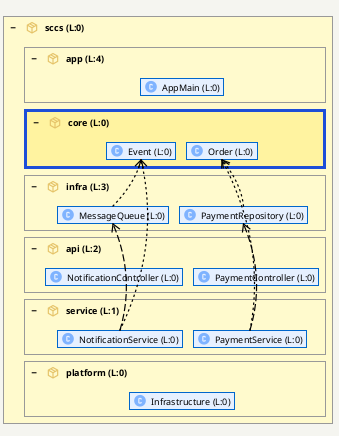
\includegraphics[width=0.45\textwidth]{figures/whatif-core-over-infra.png}
  \caption{What-if move: package \texttt{core} is moved from Level~0 between
  Level~3 and Level~4. This creates six violations because existing
  dependencies now run against the chosen arrangement.}
  \label{fig:whatif-core-over-infra}
\end{figure}

Figure~\ref{fig:whatif-core-over-infra} shows exactly this workflow: the manual
arrangement no longer corresponds to the order computed from the dependencies.
It can nevertheless express a desired target architecture, for example if
\texttt{core} should conceptually lie above the infrastructure. S202 therefore
does not treat this decision as an error in the representation, but makes its
cost visible: in this case, six concrete relationships would have to be
refactored or decoupled so that the dependencies again fit the chosen layering.

In addition, there is a manual CUT logic. Back edges can be marked deliberately
as planned cuts, and the tool can then check whether these cuts actually
resolve the affected SCC. The user not only sees which edge would be a
plausible break in the order, but can also verify the effect of that cut on the
cycle.

What is cut is the dependency between two classes. For every cut the tool shows
what carries it: the individual method calls, and the other references~--
fields, parameters, casts~-- that keep the dependency alive even when every call
has been removed. A cycle often arises from a few concrete places in the code,
not from the entire domain relationship between two classes; the tool names
these places and thereby the effort a cut stands for.

\section{Implementation at the Conceptual Level}

The implementation deliberately separates the computation into several
phases. The decisive point is that no phase fixes a visible position before the
information that justifies this position is available.

\begin{enumerate}
  \item \textbf{Build the class graph:} A directed class graph is created from
        the bytecode. This graph remains the raw domain model of the analysis.
        Edges of every kind enter the ordering computation:
        \texttt{extends}, \texttt{implements}, \texttt{imports},
        \texttt{instantiates}, \texttt{calls}, inheritance with a nested class
        at one end, and pure type references (\texttt{uses}). Nested classes
        count for the class that encloses them.
  \item \textbf{Detect SCCs:} Strongly connected components are determined on
        the class graph using Tarjan. The result is not yet a layout, but the
        information which classes can be ordered acyclically and which belong
        to cycles (red overlay).
  \item \textbf{Order the containers:} Every class dependency is projected onto
        the two children of the deepest common container and counted there as a
        weighted sibling edge. Per container, the SCCs of the sibling graph are
        recorded as tangles (orange overlay), resolved with the rank cut, and
        the remaining order is translated by longest-path into a
        \emph{localLevel} per child. The cut sibling edges are the container
        back edges.
  \item \textbf{Derive class back edges:} A class dependency is a back edge
        when its projection was cut. It is kept as a \emph{classBackEdge}
        finding and shown as a dashed violation edge.
  \item \textbf{Compute global levels:} The \emph{architectureLevel} of
        classes arises by longest-path on the class graph without the level
        cuts~-- the back edges inside class cycles~--, that of packages on the
        package graph of non-back-edges between different subtrees. Both
        graphs are acyclic by construction.
  \item \textbf{Check consistency:} Finally, the finished representation is
        checked redundantly against the five consistency rules.
\end{enumerate}

In short:

\begin{lstlisting}
Bytecode -> class graph -> class SCCs (red overlay)
         -> per container: sibling graph -> tangles (orange overlay)
                           -> rank cut (back edges) -> localLevel
         -> class back edges -> level cuts
         -> architectureLevel (classes, packages)
         -> consistency rules
\end{lstlisting}

\section{Conclusion}

S202 computes the most plausible hypothesis of the actual architecture from
the existing dependencies. The result is a verifiable hierarchical layered
representation: class dependencies provide the graph, every container orders
its children by exactly these dependencies, back edges make necessary breaks
visible, and consistency rules check whether the finished representation
satisfies its own claim.

A key design decision is the explicit separation of two kinds of cycles.
Class cycles and package cycles are detected independently, stored as distinct
findings, and exposed through separate toggle switches in the UI. Class cycles
(red) show which concrete classes form cyclic dependency chains;
package cycles (orange) show which packages are mutually dependent at the
architectural level. Because both views are available simultaneously, the tool
can answer two different questions at once: \emph{where} in the package
structure is the circular coupling, and \emph{which concrete class
dependencies} cause it.

The most important contribution is therefore not an optically improved graph,
but the connection of representation, explanation, and changeability. The
layering shows a possible order. The marked findings explain where this order
is broken by concrete dependencies. What-if moves and manual CUTs make visible
which refactorings can reduce these breaks or actually dissolve cycles.

This makes the visualization more than a layout. It is an explainable working
model: every position and every highlighted edge must be traceable to a
comprehensible decision in the computation, and every planned change can be
checked against the same order.

\end{document}
